\begin{frame}
  \frametitle{Validation process}
  \begin{itemize}
    \item Comparison of the results with the new method and the old one at the
      11th decimal of total energy in a few test cases with up to 100 steps
    \item Comparison of various intermediates quantities on the first iterations
    \item Comparison of the results with differents diagonalization algorithm
      for the Hamiltonian (LOBPCG, Chebychev, Conjugate gradient)
    \item Comparison of the results with differents CPU configurations
    \item Add of \texttt{paral[84]} and \texttt{paral[86]} to the testsuite
  \end{itemize}
\end{frame}

\begin{frame}
  \frametitle{Results}
  \begin{figure}[ht]
    \centering
    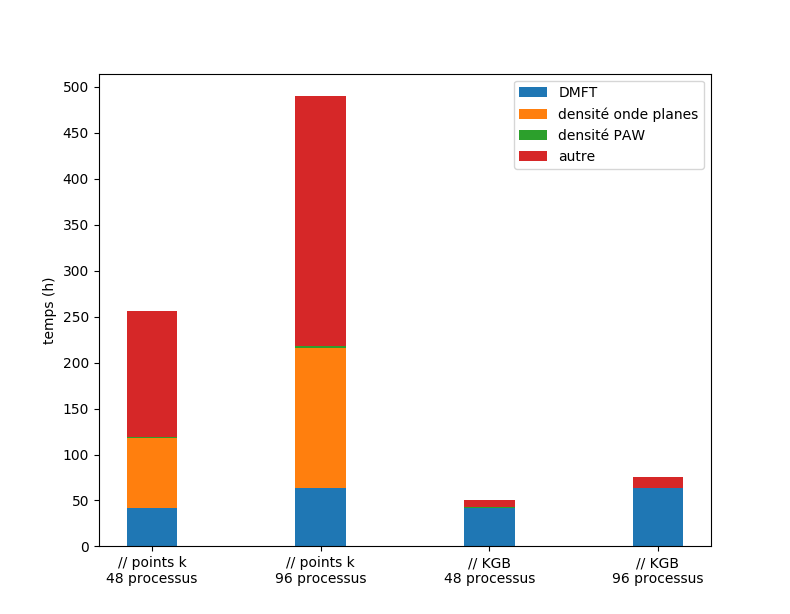
\includegraphics[width=0.7\textwidth]{pic/bargraph.png}
    \caption{Drastic effect of the use of paral\_kgb on a DMFT computation}
    \label{fig:bargraph.png}
  \end{figure}
\end{frame}
